\subsubsection{Ý tưởng}
Bubble Sort là thuật toán sắp xếp so sánh liên tiếp các cặp phần tử liền kề trong mảng và hoán đổi nếu chúng không theo đúng thứ tự. Quá trình này được lặp lại cho đến khi mảng được sắp xếp. Với mỗi lần lặp, phần tử lớn nhất (hoặc nhỏ nhất) sẽ "nổi" lên cuối (hoặc đầu) mảng.
\subsubsection{Mã giả}

\begin{algorithm}[H]
\caption{BubbleSort}
\begin{algorithmic}[1]
\Procedure{BubbleSort}{$arr, n$}
    \State \textbf{Input:} Mảng $arr$ gồm $n$ phần tử
    \State \textbf{Output:} Mảng $arr$ được sắp xếp
    
    \For {$i \gets 0 $ \textbf{to} $n$}
        \For {$j \gets 0$ \textbf{to} $n - i - 1$} 
            \If{$arr[j] > arr[j+1]$}
                \State \textbf{swap} $arr[j]$ \textbf{and} $arr[j+1]$
            \EndIf
        \EndFor
    \EndFor
\EndProcedure
\end{algorithmic}
\end{algorithm}

\subsubsection{Ví dụ}

\begin{figure}[H]
    \centering
    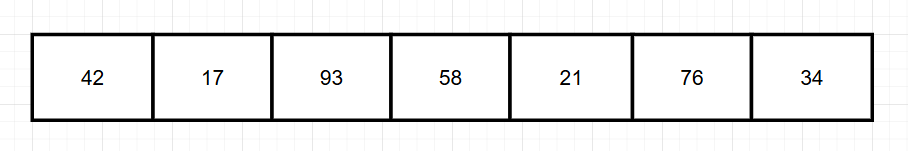
\includegraphics[width=1\linewidth]{img/bubble_sort/1.png}
    
    \vspace{0.5cm}
    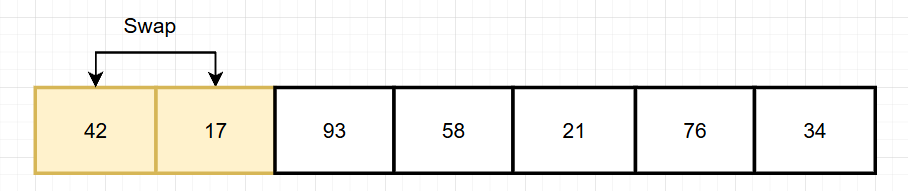
\includegraphics[width=1\linewidth]{img/bubble_sort/2.png}
    \vspace{0.5cm}
    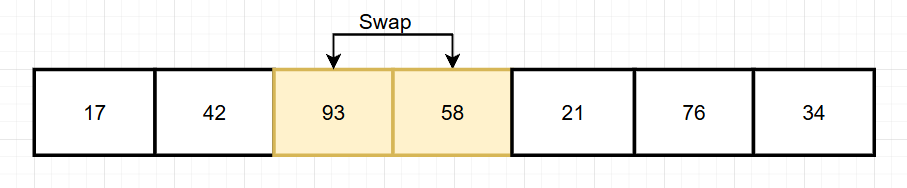
\includegraphics[width=1\linewidth]{img/bubble_sort/3.png}
    \vspace{0.5cm}
    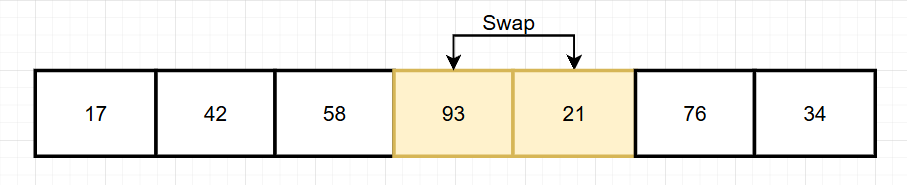
\includegraphics[width=1\linewidth]{img/bubble_sort/4.png}
    \vspace{0.5cm}
    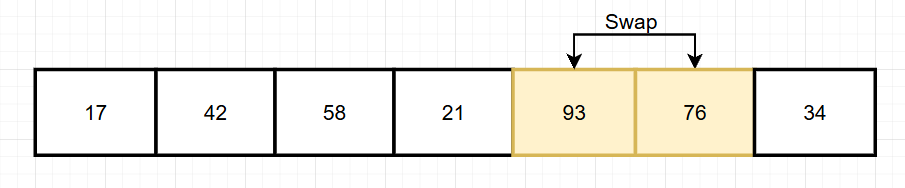
\includegraphics[width=1\linewidth]{img/bubble_sort/5.png}
    \caption{Các bước chạy - 1}
    \label{fig:part1}
\end{figure}

\begin{figure}[H]
    \centering
    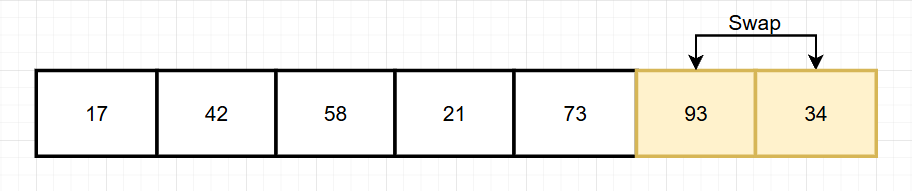
\includegraphics[width=1\linewidth]{img/bubble_sort/6.png}
    
    \vspace{0.5cm}
    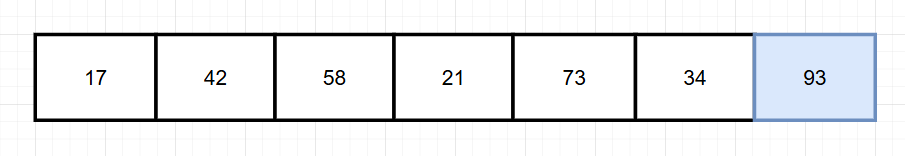
\includegraphics[width=1\linewidth]{img/bubble_sort/7.png}
    \vspace{0.5cm}
    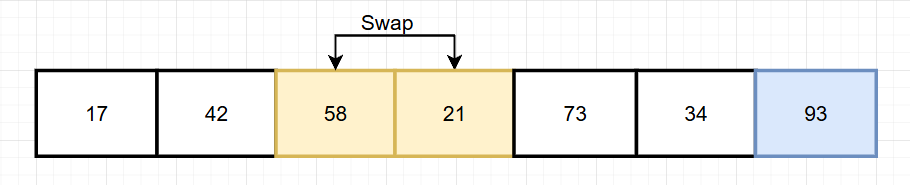
\includegraphics[width=1\linewidth]{img/bubble_sort/8.png}
    \vspace{0.5cm}
    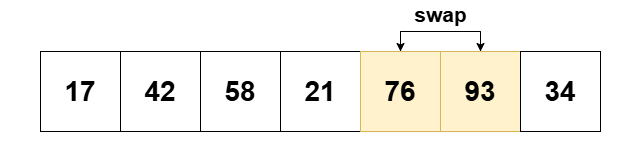
\includegraphics[width=1\linewidth]{img/bubble_sort/9.png}
    \vspace{0.5cm}
    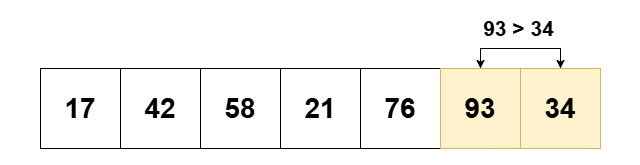
\includegraphics[width=1\linewidth]{img/bubble_sort/10.png}
    \caption{Các bước chạy - 2}
    \label{fig:part2}
\end{figure}

\begin{figure}[H]
    \centering
    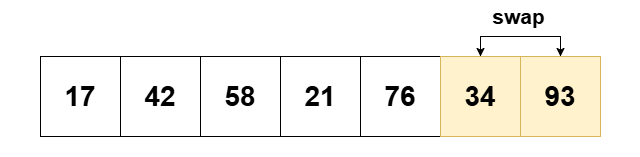
\includegraphics[width=1\linewidth]{img/bubble_sort/11.png}
    
    \vspace{0.5cm}
    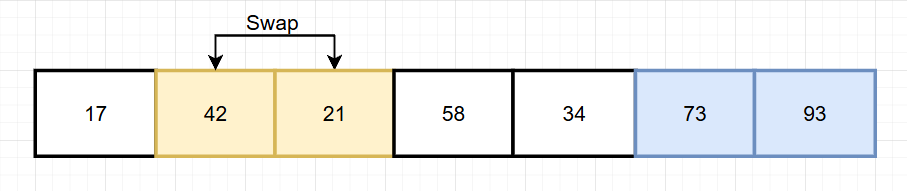
\includegraphics[width=1\linewidth]{img/bubble_sort/12.png}
    \vspace{0.5cm}
    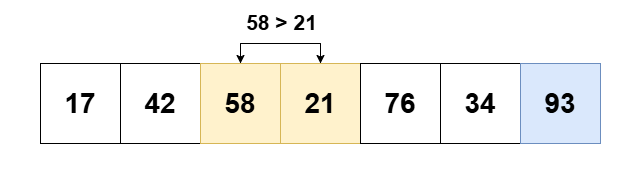
\includegraphics[width=1\linewidth]{img/bubble_sort/13.png}
    \vspace{0.5cm}
    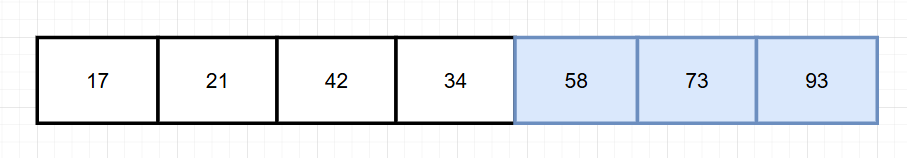
\includegraphics[width=1\linewidth]{img/bubble_sort/14.png}
    \vspace{0.5cm}
    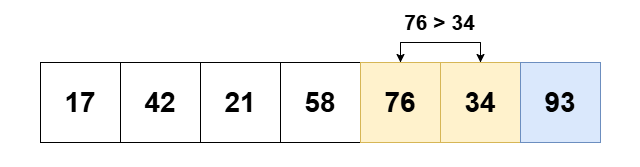
\includegraphics[width=1\linewidth]{img/bubble_sort/15.png}
    \caption{Các bước chạy - 3}
    \label{fig:part3}
\end{figure}

\begin{figure}[H]
    \centering
    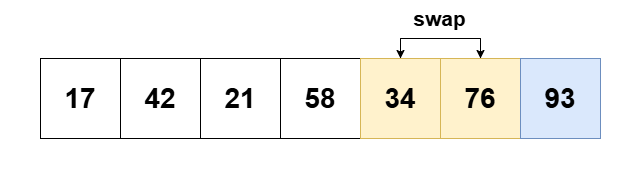
\includegraphics[width=1\linewidth]{img/bubble_sort/16.png}
    
    \vspace{0.5cm}
    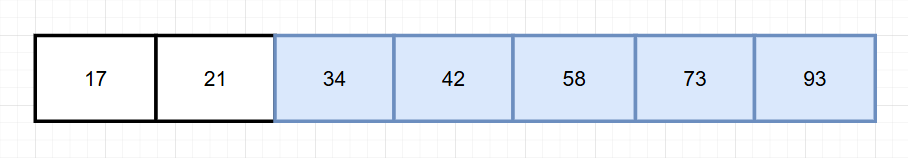
\includegraphics[width=1\linewidth]{img/bubble_sort/17.png}
    \vspace{0.5cm}
    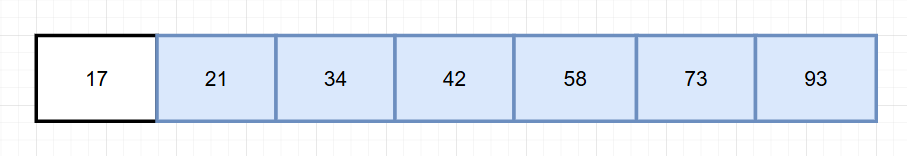
\includegraphics[width=1\linewidth]{img/bubble_sort/18.png}
    \vspace{0.5cm}
    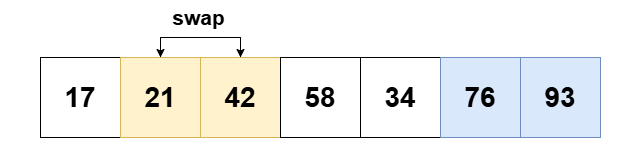
\includegraphics[width=1\linewidth]{img/bubble_sort/19.png}
    \caption{Các bước chạy - 4}
    \label{fig:part4}
\end{figure}


\subsubsection{Độ phức tạp}